\subsection{Teilsysteme von Kraftfahrzeugen}
Moderne Kraftfahrzeuge werden aus folgenden Teilsysteme gebildet:
\begin{itemize}
	\item Antriebseinheit
	\item Energieübertragungseinheit
	\item Stütz- und Trageeinheit
	\item Steuerungs- und Regelungseinheit
	\item Arbeitseinheit
\end{itemize}


\begin{figure}[!ht]
	\caption{Teilsysteme des Kraftfahrzeugs}
	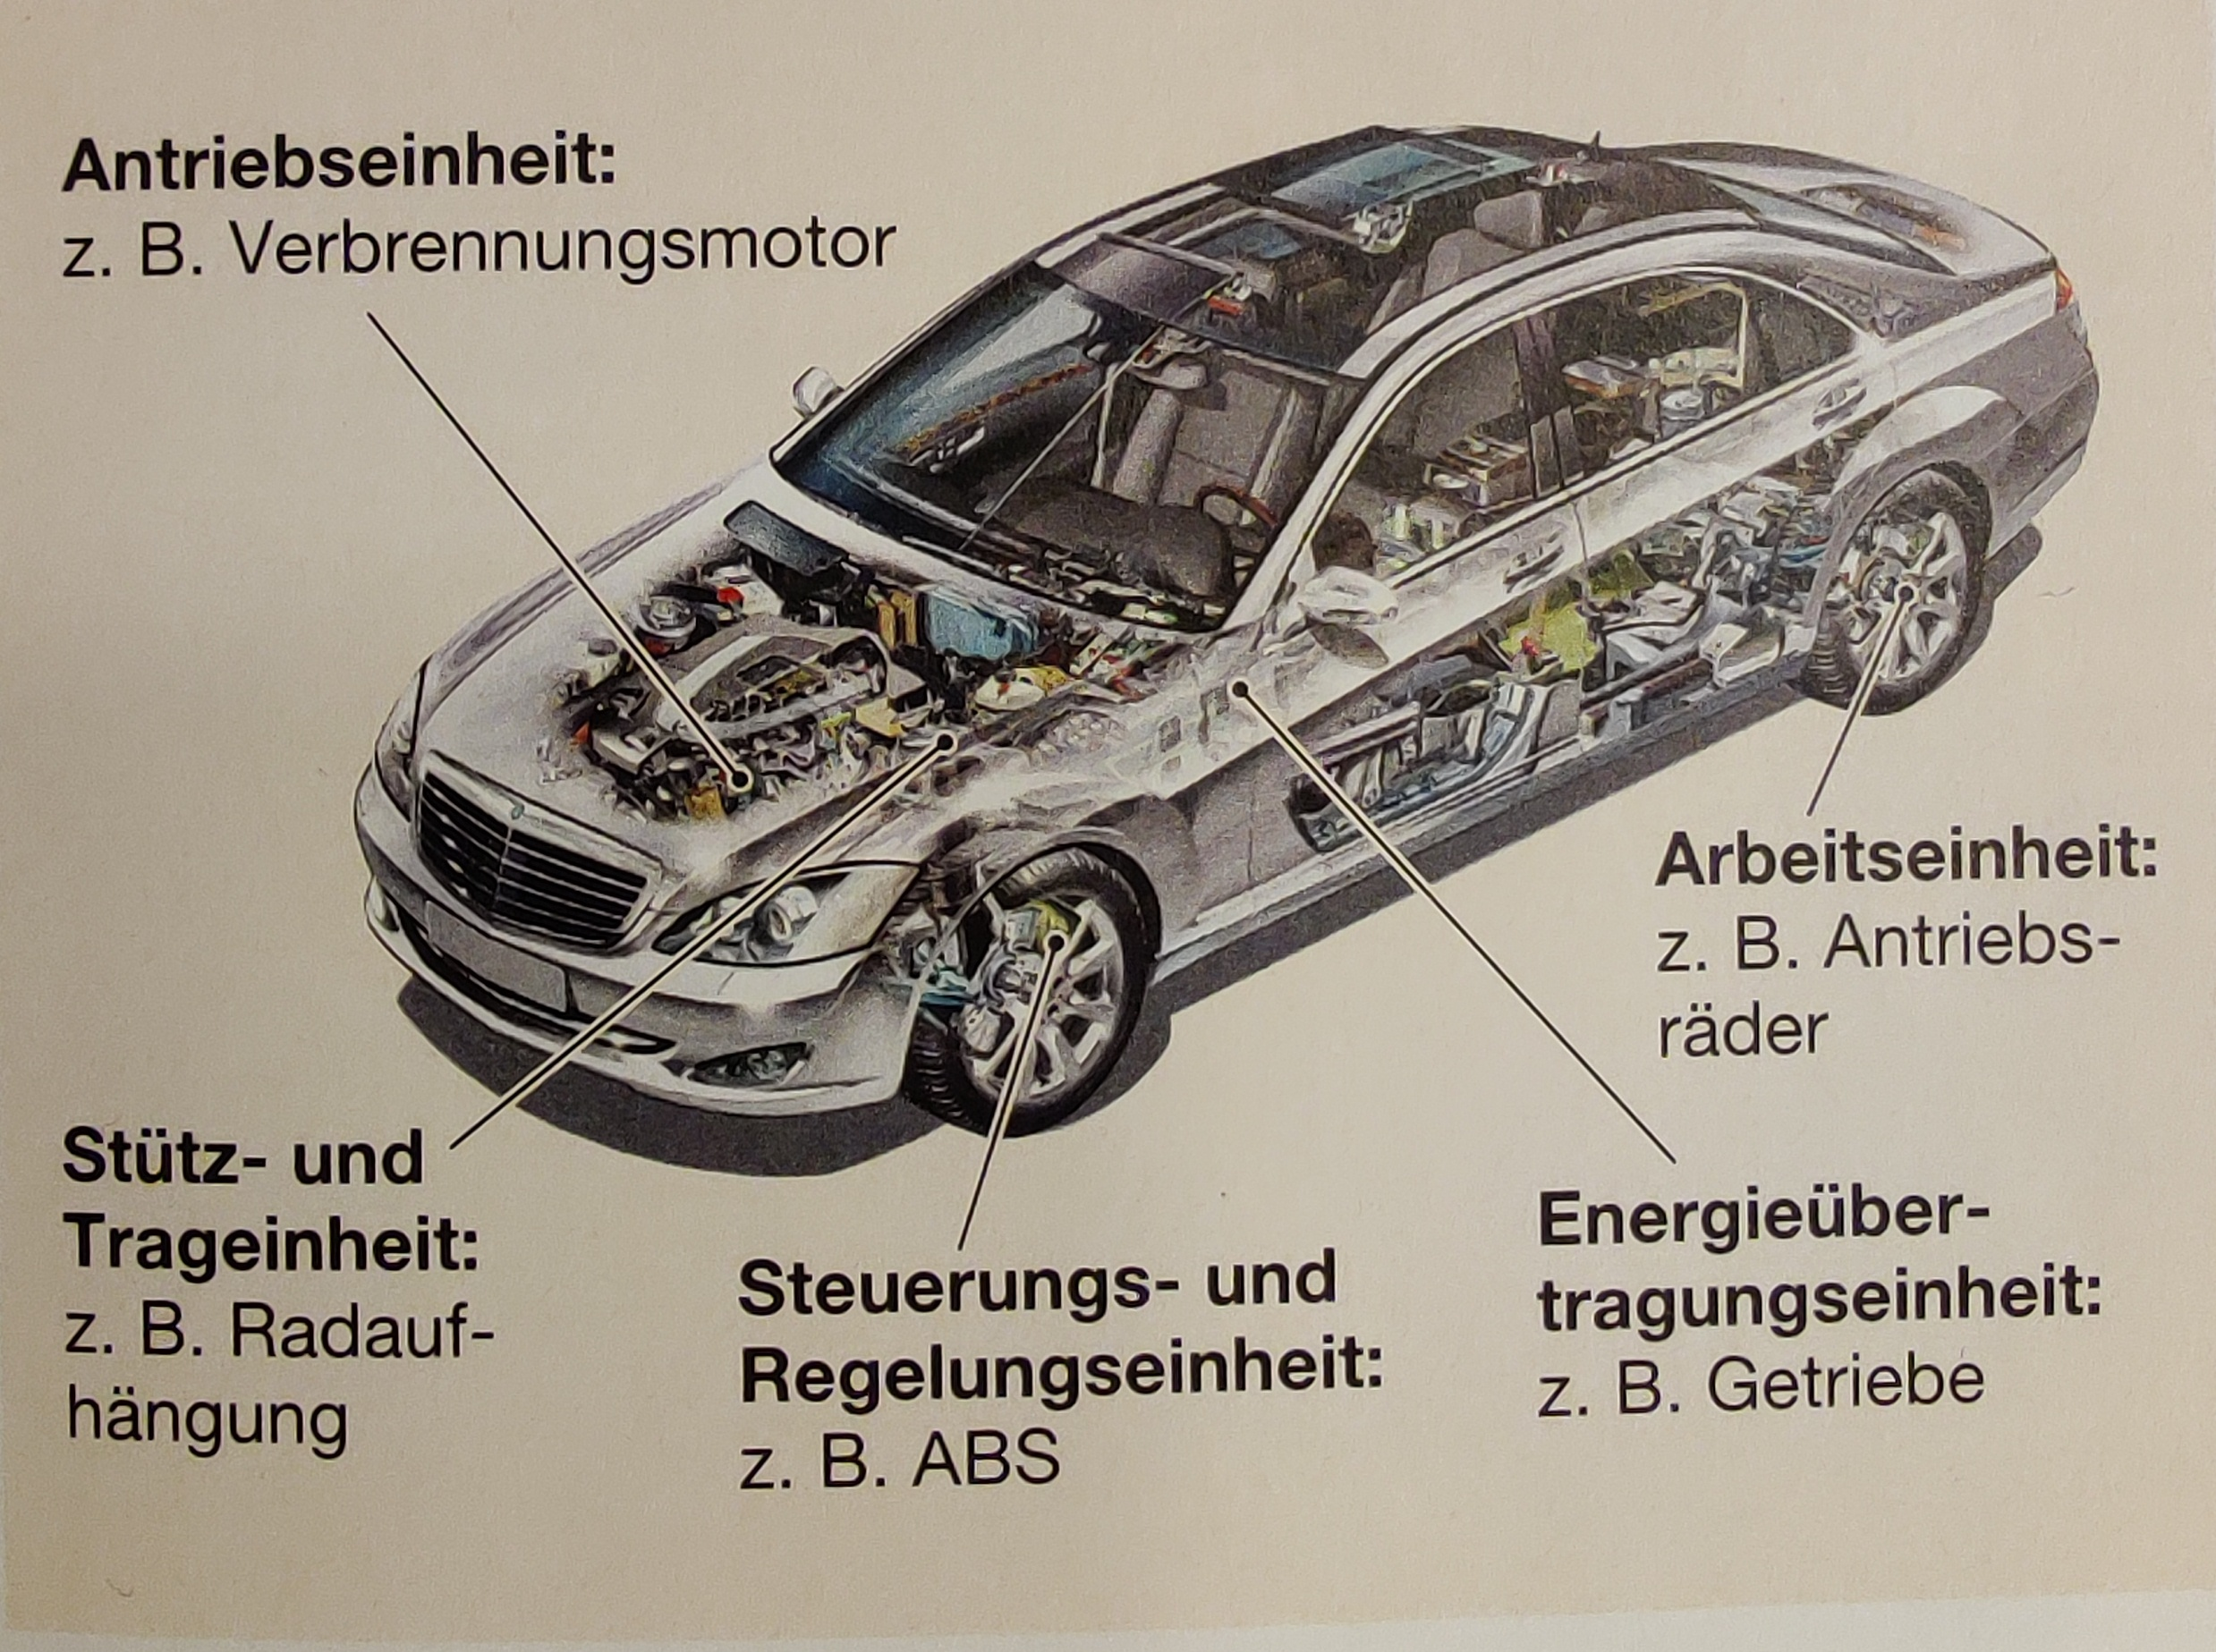
\includegraphics[scale=0.1]{assets/figures/Teilsysteme des Kraftfahrzeugs.jpg}
	\begin{flushleft}
		Quelle: Westermann S. 19
	\end{flushleft}
	\label{fig:birds}
\end{figure}


\subsubsection{Antriebseinheit}
Die Antriebseinheit wandelt die zugeführte Energie in die erforderliche Antriebsenergie um.
Diese Umwandlung wird im Motor durchgeführt.
Hauptsächlich werden Elektro- und Verbrennungsmotoren eingesetzt.

Verbrennungsmotoren unterscheiden sich von Elektromotoren durch ihre Energieerzeugung.
Die Energieerzeugung wird durch die Verbrennung von Kraftstoff erzeugt.
Dazu wird ein Kraftstoff-Luft-Gemisch in einem Brennraum mit Kolben zur Verbrennung verwendet.
Durch die Verbrennung steigt der Druck im Brennraum stark an und bewegt einen Kolben.

\subsubsection{Arbeitseinheit}
Die Arbeitseinheit ist die Verbindung zwischen den Antriebsrädern und der Fahrbahn.
Durch die Bewegung der Antriebsrädern wird das Kraftfahrzeug in Bewegung gesetzt.

\subsubsection{Energieübertragungseinheit}
Die Energieübertragungseinheit leitet die Energie in der geforderten Bewegungsart und Bewegungsgeschwindigkeit zu der Arbeitseinheit weiter.

Energieübertragungseinheiten sind Baugruppen einer Maschine, die zur Übertragung von Energie benötigt werden.
Beispiel hierfür sind Kabel die elektrische Energie leiten oder Wellen, Zahnräder und Riemen die mechanisches Drehmoment übertragen.

\subsubsection{Stütz- und Trageeinheit}
Der Rahmen oder der selbsttragende Aufbau eines Kraftfahrzeuges ist die Stütz- und Trageeinheit.
Diese haben hauptsächlich die Aufgabe, die Teilsysteme aufzunehmen und zu einer Einheit zu verbinden.

\subsubsection{Steuerungs- und Regelungseinheit}
Die Steuerungs- und Regelungseinheit beeinflusst die Stoff- und Energieumsetzung durch Informationsverarbeitung.

\subsubsection{Steuerungseinheit}
Bei der Steuerungseinheit werden verschiedene Eingangsgrößen durch das System in eine oder mehrere Ausgangsgrößen verändert.
Beispiele für Steuerungen sind:
\begin{itemize}
	\item Klimaanlage: Es wird eine Solltemperatur eingestellt.
	      Die Klimaanlage kühlt konstant.
	      Die Klimaanlage kühlt solange mit dieser eingestellten Temperatur solange sie nicht verändert wird.
	      Die Umgebungstemperatur wird nicht berücksichtigt.
	\item Licht: Der Schalter wird betätigt und das Licht wird eingeschaltet.
	      Das Licht bleibt permanent eingeschaltet.
	      Das Licht geht erst aus wenn der Schalter ausgeschaltet wird.
	      Das Umgebungslicht wird nicht berücksichtigt.
\end{itemize}

\subsubsection{Regelungseinheit}
Bei einer Regelungseinheit werden die Eingangsgrößen mit einem Sollwert verglichen und so lange angepasst bis der Sollwert erreicht wird.
Beispiele für Regelungen sind:
\begin{itemize}
	\item Klimaautomatik: es wird eine Solltemperatur eingestellt.
	      Es wird gemessen wie warm oder wie Kalt die Temperatur ist.
	      Sollte die Temperatur unter der Solltemperatur liegen, wird die Klimaautomatik auf Heizen gestellt.
	      Sollte die Temperatur über der Solltemperatur liegen, wird die Klimaautomatik auf Kühlen gestellt.
	\item Lichtautomatik: Es gibt eine Schwelle bei der das Licht eingeschaltet werden soll.
	      Es gemessen wie hell das Umgebungslicht ist.
	      Sollte das Umgebungslicht zu gering sein wie zum Beispiel im Tunnel oder bei Dämmerung wird das Licht eingeschaltet.
	      Sobald das Umgebungslicht wieder hell genug ist zum Beispiel beim verlassen des Tunnels oder bei Sonnenaufgang, wird das Licht wieder ausgeschaltet.
\end{itemize}
